\subsection{Merge Sort}

\begin{figure}[h]
	\centering
	\mbox{
		\subfigure[Test results from Merge Sort when run in .NET.]{
			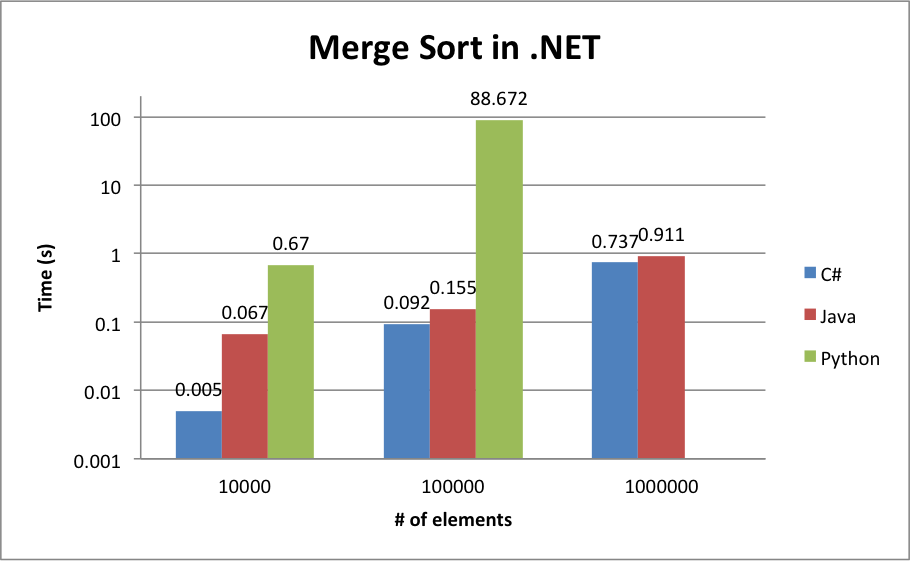
\includegraphics[width=0.48\textwidth]{chapters/media/merge_sort_all_net.png}
			\label{fig:merge_sort_all_net}
		}
		\subfigure[Test results from Merge Sort when run in native environments.]{
			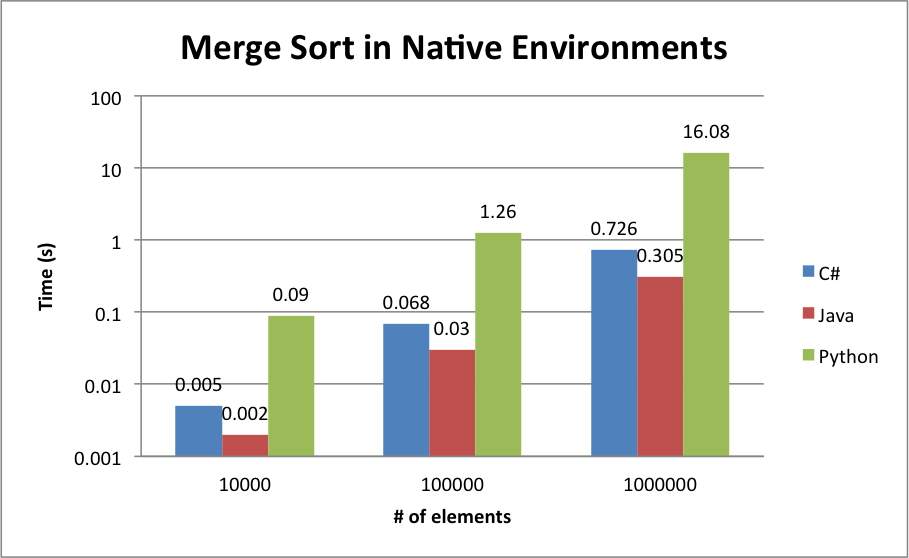
\includegraphics[width=0.48\textwidth]{chapters/media/merge_sort_all_native.png}
			\label{fig:merge_sort_all_native}
		}
	}
	\caption{Comparison of running Merge Sort in .NET to the left and each language native environment to the right.}
	\label{fig:merge_sort_net_native}
\end{figure}


Running code in its native environment provides a significant increase in performance for Merge Sort as well, see Figure \ref{fig:merge_sort_net_native}. This gap seemed to get narrower when increasing the amount of numbers to be sorted.

C\# still outperforms Java when run in the .NET environment. But the gap between them seemed to narrow the more elements were added (see Figure \ref{fig:merge_sort_all_net}). 

\begin{figure}[h]
	\centering
	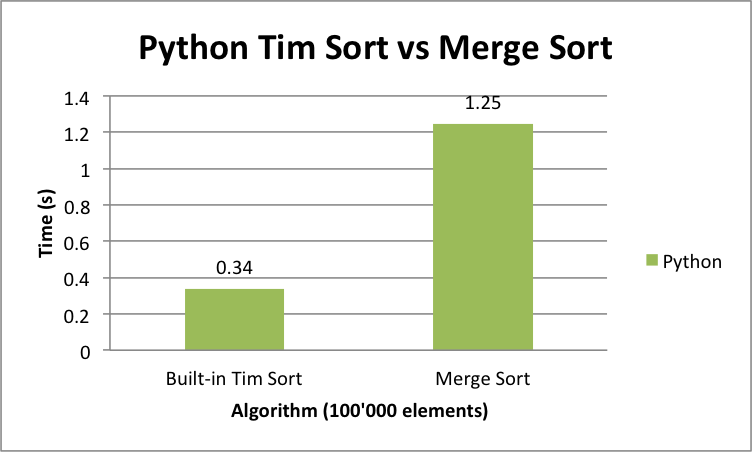
\includegraphics[width=0.6\textwidth]{chapters/media/tim_sort.png}
	\caption{Python built-in function Tim Sort vs Merge Sort.}
	\label{fig:tim_sort}
\end{figure}

Figure \ref{fig:tim_sort} illustrates the performance gained from using the built-in Python sorting function Tim Sort natively. 



\begin{figure}[h]
	\centering
	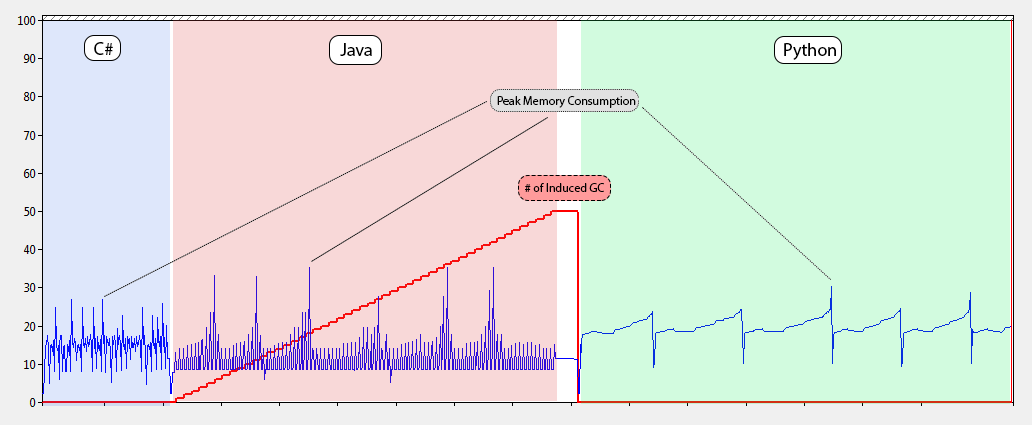
\includegraphics[width=1.0\textwidth]{chapters/media/mergesort_memory_1mil_all.png}
	\caption{Memory consumption over 100 test runs with one million elements for each language. Blue line represent memory consumption and red line represents the number of induced GC.}
	\label{fig:merge_sort_memory_all}
\end{figure}


Figure \ref{fig:merge_sort_memory_all} illustrates 100 runs with one million elements of the Merge Sort algorithm with each language run in .NET (all Python runs are not visible). It would appear that since the algorithm runs on the same input each run, one would expect a pattern to emerge. Because of restrictions in the Microsoft Performance Monitor it could only take one sample every second, and since C\# and Java ran faster than that, the plot is uneven.  This restriction makes it necessary only to consider the peak for each language. Several more runs were made in order to reduce the risk of data collection error, Figure \ref{fig:merge_sort_memory_all} is just an example run with all languages present to illustrate their differences (see Figure \ref{fig:merge_sort_memory} for  maximum values). The red line is the number of times the garbage collector was induced, note that Java forces this induction every other run.


\begin{figure}[h]
	\centering
	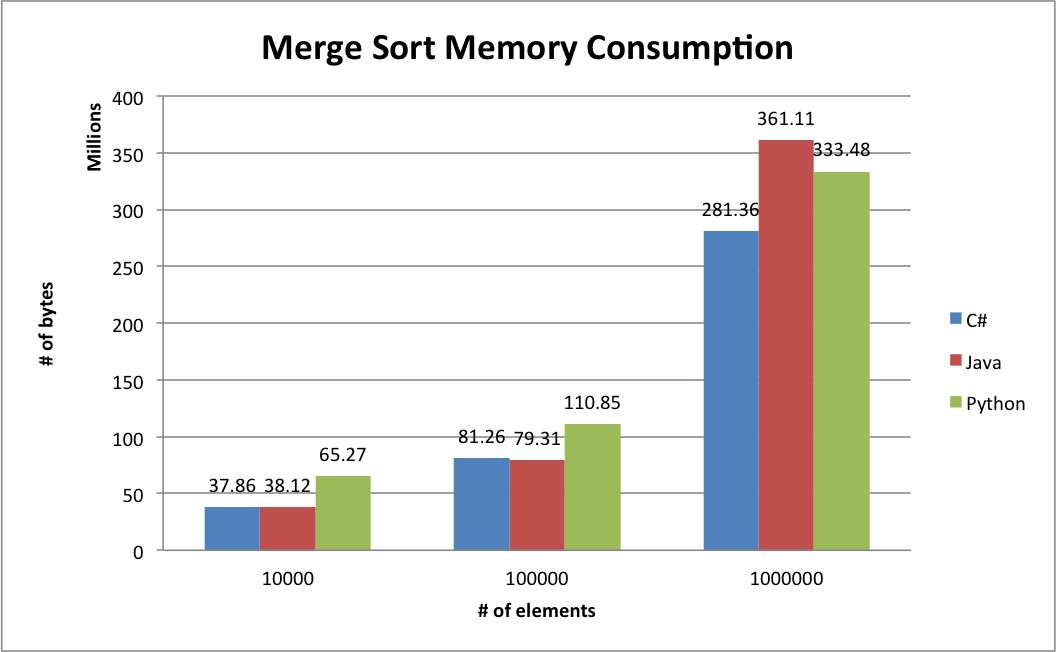
\includegraphics[width=1.0\textwidth]{chapters/media/merge_sort_memory.png}
	\caption{Comparison of the memory consumption between the three languages.}
	\label{fig:merge_sort_memory}
\end{figure}

The maximum memory consumption can be seen in Figure \ref{fig:merge_sort_memory}. Java consumed the most memory while C\# consumed the least.

























